\section{Introduzione}

Il glucosio è fondamentale per la vita degli essere umani. Risulta essere la principale fonte energetica per la gran parte degli organismi viventi fornendo fino a 285 kilocalorie per mole. 

L'organismo umano provvede ad una stretta regolazione dell'omeostasi del glucosio mantenendo i livelli di glicemia quanto più constanti possibile. Tali valori vengono alterati da diversi stimoli e l'integrazione di numerosi meccanismi di controllo porta a ristabilire le condizioni fisiologiche.
Tra questi sistemi i più importanti sono regolati dal pancreas e dal fegato.
Il fegato ha una capacità di immagazzinare glucosio piuttosto limitata ed eventuali carboidrati in eccesso vengono convertiti in grassi e depositati nel tessuto adiposo. 

A partire dalle pareti intestinali, dopo l'ingestione, il glucosio viene assorbito e indiritazzato al sistema nervoso centrale e poi al fegato e muscoli, dove viene accumulato come glicogoneo. 
L'interazione della parte endocrina del pancreas con il fegato e gli altri sistemi provvede ad una stretta regolazione della glicemia e tale processo può essere descritto tramite diversi modelli matematici.

A seguire viene analizzato il modello minimo del glucosio e le diverse possibilità che offre quali la predizione dell'eveoluzione della glicemia nel tempo, ad esempio in un test IVGGT, o l'identificazione di parametri di interesse clinico quali la glucose effectiveness o l'insulin sensitivity. 

\section{Background}

\begin{figure*}[t!]
	\centering
	\scriptsize{\def\svgwidth{0.95\linewidth}
		\input{blood_sugar.pdf_tex}}
	\caption{Sistema di regolazione della glicemia. Lo schema è semplificato rispetto la reale complessità del meccanismo di regolazione.}
	\label{fig:glucoseregolation}
\end{figure*}


\begin{figure}[b!]
	\centering
	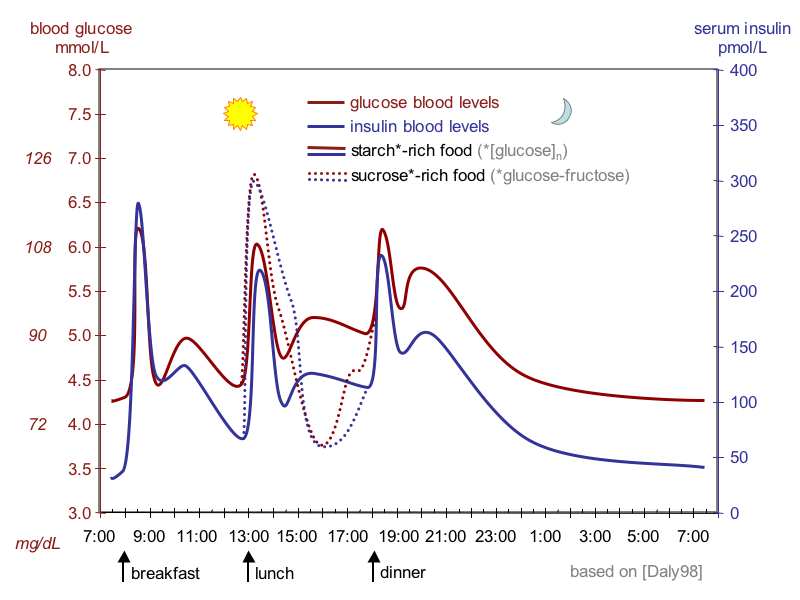
\includegraphics[width=0.99\linewidth]{figures/glucose_regolation2}
	\caption{Curva idealizzata dell'andamento di glucosio e insulina nel sangue durante il giorno, considerando tre pasti indicati dalle frecce \cite{daly_acute_1998}}
	\label{fig:glucoseregolation2}
\end{figure}

La regolazione fisiologica del glucosio è molto complessa. Il corpo integra differenti sistemi e vie di controllo per mantenere i livelli di glicemia, lontano dai pasti, ad un valore fisiologico di $80\div 90$ mg/dl.

La glicemia è la misura della concentrazione di glucosio nel sangue. Viene fortemente regolata dal corpo ed è uno dei parametri più importanti dell'omeostasi dell'organismo. 

Normalmente, il glucosio viene conservato all'interno dei muscoli e nel fegato sottoforma di glucogeno. Tale deposito consente quindi di mantenere costante la glicemia tramite differenti vie di controllo.

Il valore di glicemia può variare notevolmente in presenza di forti stimoli, ad esempio dopo un pasto ricco può crescere fino a $200\div 250$ mg/dl.

La crescita dei livelli plasmatici di glucosio porta all'attivazione di numerosi meccanismi. I due più importanti, per il ripristino dei valori di riposo, segue al rilascio nel sangue di insuline da parte delle cellule beta del pancreas. Si innescano diversi meccanismi a cascata che portano a due azioni principali:
\begin{itemize}
	\item Aumento del consumo metabolico di glucosio da parte delle cellule del corpo
	\item Stimolazione dell'uptake di glucosio nel fegato con conseguente accumulo sotto forma di glicogeno
\end{itemize}

La presenza dello stimo opposto, quale la riduzione della glicemia porta invece all'attivazione delle cellule del pancreas che a loro volta rilasciano glucagone. Tale ormone a sua volta stimola il fegato a rilasciare glucosio e si avrà un aumento del livello plasmatico di glucosio \cite{sherwood_fisiologia_2008}.

Complessivamente sono presenti differenti ormoni catabolici come il glucagone, il cortisolo e le catecolamine che portano ad un aumento della glicemia ma un solo ormone anabolico, l'insulina \cite{nelson_lehninger_2021}.

Tali meccanismi vengono alterate in alcune patologie. 
Si parla di iperglicemia quando il livello di glucosio nel sangue rimane troppo elevato. Il mantenimento di condizioni di iperglicemia per molto tempo può portare a differenti problemi di salute quali disturbi al cuore, cancro, problemi agli occhi e ai reni. 

Livelli di glucosio sopra 300 mg/dl portano a danni fatali dovuti alla chetoacidosi

Una patologia caratteristica è il diabete mellito dove si ha un'alterazione in punti differenti: nel tipo I sono le cellule beta che non riescono a far partire il rilascio di insulina, nel tipo II, invece, l'insulina non è efficace.

Anche bassi livelli di glucosio nel sangue possono portare a differenti problemi quali letargia e alterazione di alcune peculiarità neurologiche come irritabilità, debolezza e perdita di coscienza.

Si parla di ipoglicemia quando il livello è sotto i 40 mg/dl.

A tal proposito, in clinica, si utilizza un test paziente specifico, il IVGTT \cite{darden_predicting_2020-1}. Tale test, sotto il nome di \textit{intra venous glucose tolerance test}, permette di stimare due parametri di interesse quali:

\begin{itemize}
	\item \textit{glucose effectiveness}, il glucosio stesso ha un effetto sulla riduzione della glicemia
	\item \textit{insulin sensitivity}, misura l'efficacia dell'insulina nel ridurre i livelli plasmatici di glucosio
\end{itemize}

Si contrappone a test più veloci come il test orale OGTT e presenta una precisione notevolmente maggiore per la prima fase (fase acuta) di rilascio dell'insulina. Viene iniettato glucosio per via venosa e questo permette di evitare il sisitema digestivo e quindi di avere una maggiore sensibilità.

Quando le cellule $\beta$-pancreatiche rilasciano insulina nella vena portale, passa nel fegato e viene parzialmente eliminata prima di entrare in circolazione. Inoltre, il tasso di clearance dell'insulina epatica può variare per meccanismi sia fisiologici che farmagolici. Quindi, la concentrazione di insulina misurata nei vasi periferici può essere fortemente diversa da quella rilasciata dal pancreas.

Il test IVGTT richiede una modello matematico per stimare i parametri e viene spesso utilizzato il modello minimo del glucosio che permette di stimare la risposta pancreatica e la sensibilità insulinica. Si deve precisare anche che il corretto svolgimento di un test IVGTT richiedere personale qualificato in grado anche di applicare una modellazione matematica \cite{cersosimo_assessment_nodate}. 

Il test può durare diverse ore e vengono raccolte le concentrazione del rilascio di glucosio e della concentrazione di insulina o, alternativamente, il C-peptide. Nelle sezioni seguente non si analizzano i modello a C-peptide ma si considera la concentrazione di insulina misurata nel sangue.





\begin{figure}[t!]
	\centering
		\scriptsize{\def\svgwidth{0.95\linewidth}
		\input{minimal.pdf_tex}}
	\caption{Schema a blocchi del modello minimo del glucosio}
	\label{fig:modellominimo}
\end{figure}


\subsection{Modello minimo del glucosio}



Il modello minimo del glucosio è un modello matematico che permette di descrivere l'evoluzione della concentrazione plasmatica di glucosio. 

Come ogni modello, si deve trovare un compromesso tra l'accuratezza, l'affidabilità, il costo computazionale e il numero dei parametri da stimare per poterlo utilizzare. 

Questo modello, come indicato dal nome, utilizza il numero minore di parametri possibile per poter avere una descrizione sufficientemente accurata da permettere la valutazione delle due quantità clinicamente interessanti, quali la glucose effectiveness e la glucose sensitivity. 

Tale modello è stato introdotto da Bergman e Cobelli \cite{bergman_quantitative_1979} e prevede la suddivisione in due compartimenti (\cref{fig:modellominimo}), rappresentati da due equazioni differenziali:

\begin{equation}
	\begin{cases}\frac{d G}{d t}=S_{g}\left(G_{b}-G\right)-X G, & \mathrm{G}(0)=G_{0} \\ \frac{d X}{d t}=k\left[S_{i}\left(I-I_{b}\right)-X\right], & \mathrm{X}(0)=X_{0}\end{cases}
	\label{eq:modello}
\end{equation}

Il primo compartimento rappresenta la concentrazione plasmatica di glucosio $G(t)$ variabile nel tempo. Viene influenzata dalla concentrazione di glucosio stessa in due differenti modalità. Per il tramite della glucose effectiveness $S_g$ si ha un verso di crescita proporzionale alla differenza tra la concentrazione basale e quella attuale, si osservi che tale differenza diventa negativa per cui più cresce il divario, rispetto la concentrazione basale, più il glucosio tenderà a diminuire. 

\begin{figure*}[t!]
	\begin{subfigure}{0.5\linewidth}
		\centering
		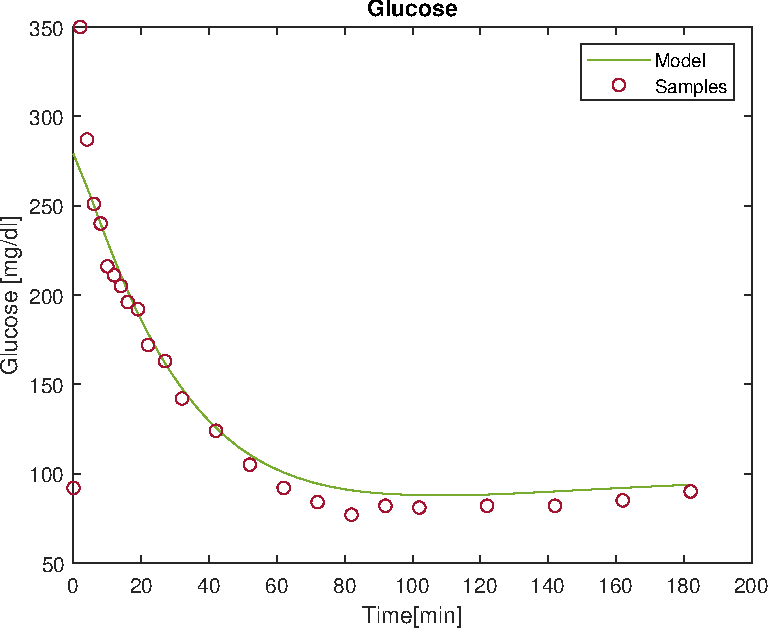
\includegraphics[width=0.95\linewidth]{../code/prediction/matlab/figs/glucose_model}
		\caption{}
		\label{fig:glucosemodel}
	\end{subfigure}\hfill
	\begin{subfigure}{0.5\linewidth}
		\centering
		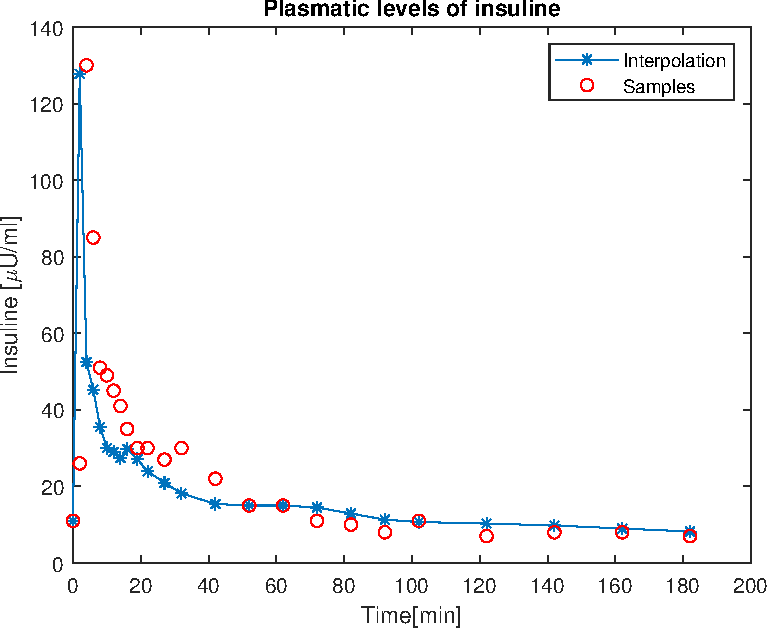
\includegraphics[width=0.95\linewidth]{../code/prediction/matlab/figs/insuline_model}
		\caption{}
		\label{fig:insuline_model}
	\end{subfigure}\hfill
	\caption{Andamento nel tempo della concentrazione di glucosio (a) e dell'insulina (b) nel sangue. Per il glucosio sono presenti i campioni (dai dati numerici) rappresentati con i cerchietti e la linea continua rappresentante la soluzione predetta. Per l'insulina sono presenti i campioni rappresentanti con i cerchietti e la curva ottenuta con l'interpolazione lineare valutata negli stessi istanti temporali.}
\end{figure*}

Il secondo termine prevede un tasso di crescita inversamente proporzionale alla concentrazione di insulina efficace $X(t)$. Tale quantità non è direttamente misurabile ma è legata al secondo compartimento e a sua volta ha un tasso di crescita influenzato da due parametri. Vi è un feedback negativo da parte della sua stessa concentrazione e un feedback proporzionale alla differenza tra la concentrazione di insulina attuale e quella basale, per il tramite di un coefficiente di proporzionalità $k\cdot S_i$, legato quindi alla insuline sensitivity $S_i$. Il tasso di crescita sarà positivo all'aumentare della concentrazione insulinica. 

Questo secondo compartimento porta in conto il fatto che il livello di insulina nel plasma raggiunge un plateau intorno ai 90 $\mu$U/ml e durante la sua evoluzione aumenta la mobilità del glucosio. 
\\

Tramite tale modello è possibile risalire ai parametri di interesse clinico, quali la glucose effectiveness e la insuline sensitivity a partire dai dati di un test IVGTT. Alternativamente, se noti i parametri descrittivi, è possibile predire l'andamento della concentrazione del modello.

A seguire vengono analizzate entrambe le possibilità sfruttando Matlab e Simulink \cite{simulink}.

\section{Predizione}

Per la predizione si considerato i parametri in \cref{tab:parametri}. 

I dati dei test possono essere presi da dati clinici o generati tramite Simulink, implementando il modello con dei coefficienti noti in letteratura \cite{pacini_minmod_1986}. 

\subsection{Soluzione ODE}



\begin{table}[t!]
	\centering
\small{
\begin{tabular}{|c|c|}
	\hline
	Variabile & Valore \\
	\hline
	$\mathtt{G0}$ & $279$ \\
	\hline
	$\mathtt{x0}$ & $0$ \\
	\hline
	$\mathtt{Gb}$ & $93$ \\
	\hline
	$\mathtt{Ib}$ & $11$ \\
	\hline
	$\mathtt{Sg}$ & $2.6\cdot 10^{-2}$ \\
	\hline
	$\mathtt{k}$ & $2.5\cdot 10^{-2}$ \\
	\hline
	$\mathtt{Si}$ & $5\cdot 10^{-4}$ \\
	\hline
\end{tabular}}
\caption{Parametri numerici utilizzati per il modello minimo del glucosio}
\label{tab:parametri}
\end{table}

\begin{figure*}[t!]
	\begin{lstlisting}[language=matlab]
		parameters=[Sg,Gb,k,Ib,Si];
		[t,y] = ode45(@(t,y) odefcn(t,y,insuline,time,parameters), [time(1), time(end)],[G0,x0]);	
	\end{lstlisting}
	\caption{Snippet della routine principale per la soluzione del sistema di equazioni differenziali in Matlab}
	\label{fig:code1}
	\vspace{0.5cm}
	\begin{lstlisting}[language=matlab]
		function dydt=odefcn(t,y,insuline,time,parameters)
		Sg=parameters(1);
		Gb=parameters(2);
		k=parameters(3);
		Ib=parameters(4);
		Si=parameters(5);
		% y(1) = G(t); 	% y(2)= X(t)
		% dGdt=Sg (Gb-G(t))-X(t)*G(t); 	
		% dXdt=k*(Si*(I(t)-Ib)-X(t)) 
		% The solver need I(t) at every t wtih linear interpolation 
		I_inter=interp1(time,insuline,t);
		dydt(1)=Sg*(Gb-y(1))-y(2)*y(1);
		dydt(2)=k*(Si*(I_inter-Ib)-y(2));
		dydt=dydt'; 
		end
	\end{lstlisting}
	\caption{Funzione contente il sistema di equazioni differenziali che verrà passato ad $\mathtt{ode45()}$ all'interno della routine principale}
	\label{fig:code2}
\end{figure*}

\begin{figure*}[t!]
	\begin{subfigure}{0.95\linewidth}
		\centering
		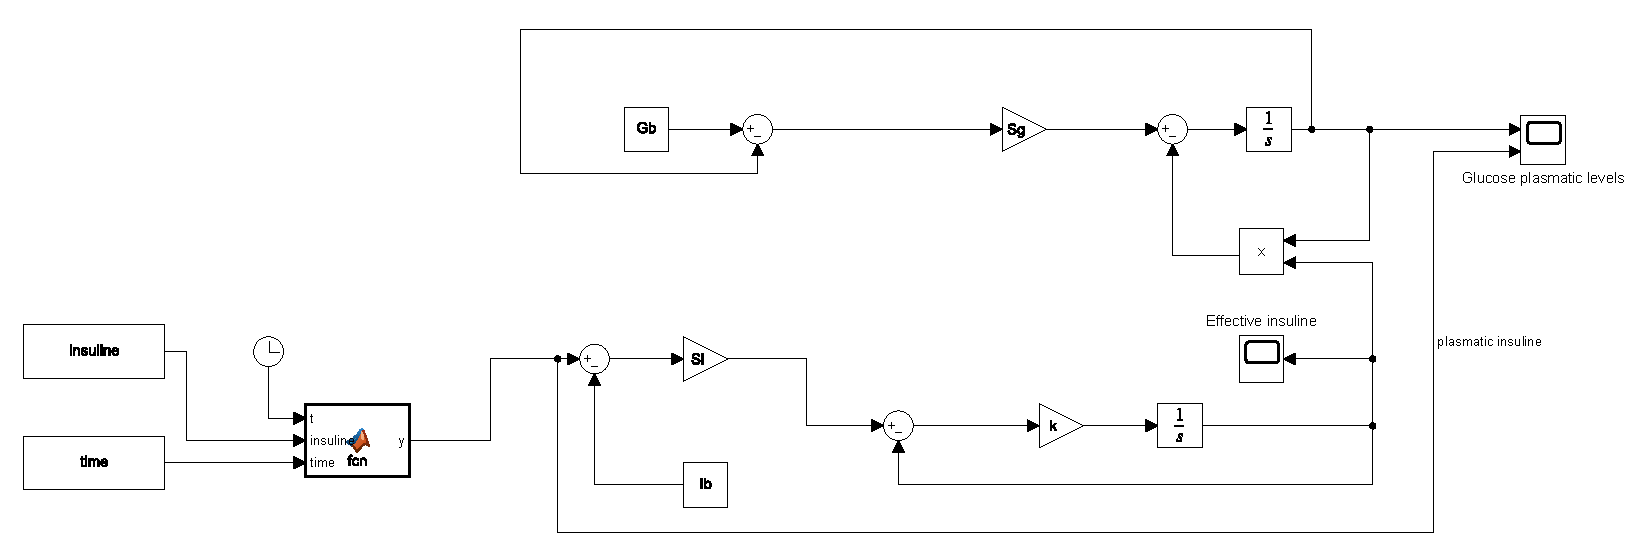
\includegraphics[width=0.85\linewidth]{figures/simulink_extended}
		\caption{}
		\label{fig:simulinkextended}
	\end{subfigure}
	\begin{subfigure}{0.95\linewidth}
		\centering
		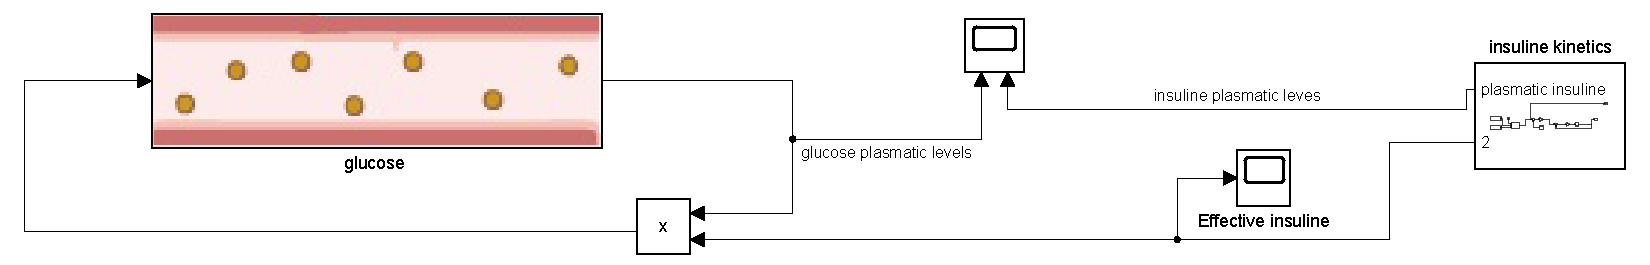
\includegraphics[width=0.85\linewidth]{figures/simulink}
		\caption{}
		\label{fig:simulinkcompact}
	\end{subfigure}
	\caption{Implementazione del sistema di equazioni differenziali descrittive il modello minimo del glucosio in versione estesa (a) e compattata mediante maschere e sotto-sistemi (b)}
	\label{fig:simulink}
\end{figure*}

A partire dai valori di insulina, campionata e presente nei dati in \cref{fig:insuline_model} è possibile implementare e risolvere il modello tramite un solutore di equazioni differenziali, \texttt{ode45()}. L'algoritimo si basa su metodo esplicito di Runge-Kutta di ordine 4 e 5 richiedendo quindi solamente la soluzione al passo precedente, oltre i parametri iniziali, e risolvendo in un singolo step temporale \cite{ode45}.

Per l'implementazione Matlab richiede di passare a \texttt{ode45()} le equazioni differenziali e i parametri. L'equazione viene passata tramite \texttt{odefcn()} mentre i parametri vengono uniti all'interno di un array \cref{fig:code1}. 

Inoltre, vengono passati i valori iniziali e il vettore dei tempi. 

Per il vettore temporale conviene passare solamente l'instante iniziale e finale lasciando l'algoritmo libero di scegliere il passo, così da avere un risultato più accurato. Tale vettore \texttt{time} fa parte dei dati sperimentali contenenti anche i campioni di glucosio, in \cref{fig:glucosemodel} utilizzati per il confronto, e di insulina, in \cref{fig:insuline_model}, utilizzati nella predizione.

Il modello matematico in \cref{eq:modello} viene quindi inserito all'interno di \texttt{odefcn()}, in \cref{fig:code2}, con l'accortezza di garantire il valore dell'insulina $I(t)$ ad ogni instante temporale. Per fare ciò si utilizza un'interpolazione lineare sui valori campionati, leggendone il valore allo stesso istante temporale utilizzato nella soluzione del sisitema di equazioni differenziali.



Il modello, una volta risolto, fornisce la curva $G(t)$ che può essere confrontata con i valori campionati (\cref{fig:glucosemodel}). 

Il modello consente di predire i valori a qualsiasi istante temporale ed in particolare con un errore medio, ad eccezione del primo campione in cui c'è una forte differenza, del 6.6\% rispetto ai campioni disponibili.


\begin{figure*}[t!]
	\begin{subfigure}{0.5\linewidth}
		\centering
		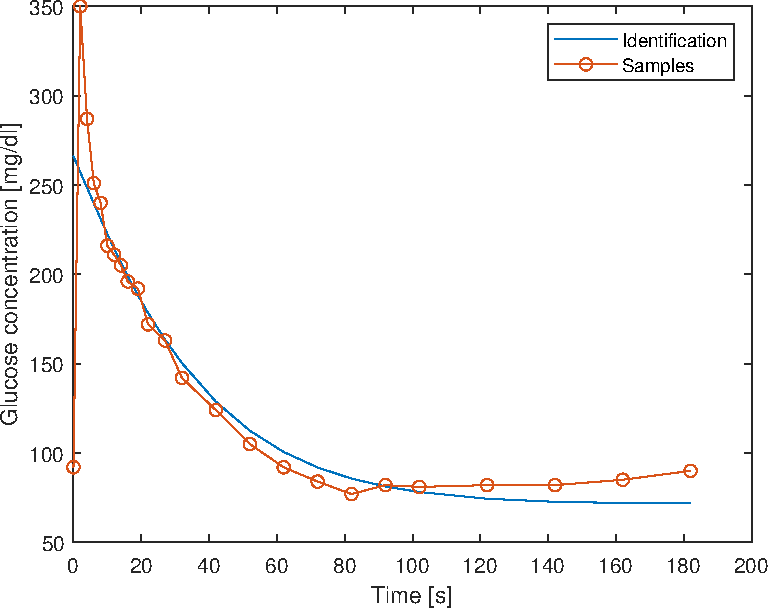
\includegraphics[width=0.95\linewidth]{../code/identification/optim}
		\caption{}
		\label{fig:optim}
	\end{subfigure}\hfill
	\begin{subfigure}{0.5\linewidth}
		\centering
		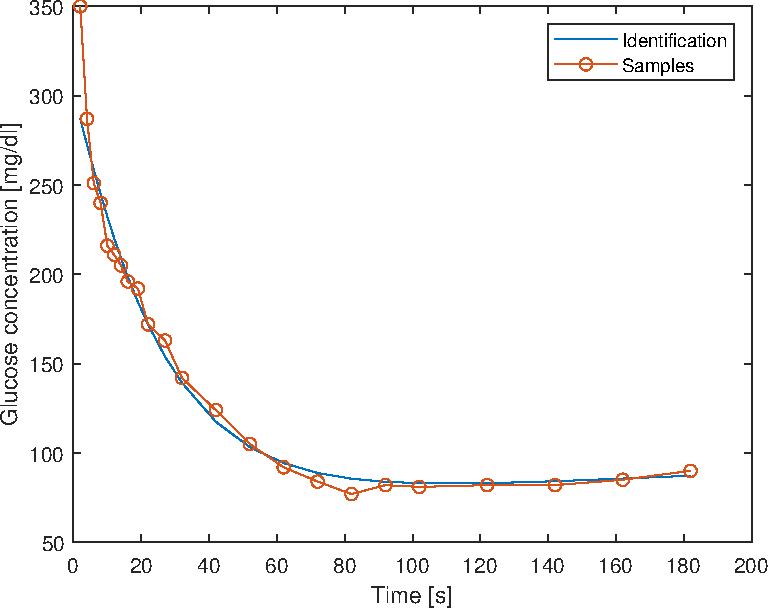
\includegraphics[width=0.95\linewidth]{../code/identification/optim1}
		\caption{}
		\label{fig:optim1}
	\end{subfigure}\hfill
	\caption{Risultato di ottimizzazione con il modello risolto con i parametri identificati e i campioni di confronto. Considerando tutti i campioni di glucosio disponibili (a), trascurando il primo (b)}
\end{figure*}

\begin{figure*}[t!]
	\begin{lstlisting}[language=matlab]
		p_init=[0.399e-1, 0.2e-1,0.4e-4,0.287e3]; 
		options = optimoptions('lsqnonlin','Display','iter');
		options.Algorithm = 'levenberg-marquardt';
		options.StepTolerance=1e-8;
		options.PlotFcn='optimplotresnorm';
		options.Display='iter-detailed';
		[x,resnorm,residual,exitflag,output,lambda,jacobian] = lsqnonlin(@optfcn,p_init,[],[],options);	
		disp(['Error: ',num2str(100*(p_true-x)./p_true),'%'])
	\end{lstlisting}
	\caption{Snippet di codice per l'impostazione del problema di ottimizzazione}
	\label{fig:code3}
\end{figure*}


\subsection{Modellazione in Simulink}

Lo stesso sistema di equazioni differenziali può essere implementato in Simulink.

Rimane necessario fornire la funzione descrittiva dell'andamento temporale dell'insulina e per farlo si può usare un blocco \texttt{Matlab function} facendo l'interpolazione lineare.



I dati dei campioni e i parametri vengono caricati tramite un file \texttt{.m}.

Per distinguere i due compartimenti è utile anche utilizzare maschere e sotto-sistemi, raggruppando i relativi componenti. Ovvero si passa da un modello esteso (\cref{fig:simulinkextended}) ad un modello compatto (\cref{fig:simulinkcompact}) e si osserva come i due compartimenti sono legati proprio dal prodotto $X(t)G(t)$. 


\section{Identificazione parametrica}



Ragionando meno in un'ottica di simulazione e focalizzandosi più sugli aspetti clinici è possibile utilizzare tale modello anche per le diagnosi.  Ovvero è possibile approcciare un'identificazione parametrica dei parametri di interesse clinico quali la glucose effectiveness e la insulin sensitivity.

In particolare, si assumono note le curve $G(t)$ e $I(t)$ (ad esempio dal test IVGTT) insieme alla concentrazione basale di glucosio $G_b$ e di insulina $I_b$ e la condizione iniziale $X_0$ e si vanno ad identificare i quattro parametri mancanti:

\begin{equation}
	\mathbf{P}=\{S_g,\:S_i,\:G_0,\:k\}
\end{equation}

L'identificazione parametrica non è altro che il tentativo di annullare la funzione errore, data dalla differenza tra i valori noti e la predizione del modello con i parametri stimati:

\begin{equation}
	\underline{e}\left(\mathbf{P}\right)=\mathtt{glucose}[t_i]-f(t_i,\mathbf{P})
\end{equation}

Ovvero è un problema di minimizzazione della funzione obiettivo definita come la norma quadra di tale funzione errore.

Per implementare la minimizzazione numerica si utilizza \texttt{lsqnonlin()}, algoritmo in Matlab per la soluzioni di problemi non lineari ai minimi quadrati \cite{lsqnonlin}. L'algoritmo utilizza il metodo Levenberg-Marquardt, un algoritmo che si pone nel mezzo tra l'algoritmo di Gauss-Newton e il metodo della discesa del gradiente.

L'algoritmo di ottimizzazione richiede un guess iniziale e vengono forniti dei valori noti in letteratura, da \citeauthor{pacini_minmod_1986} \cite{pacini_minmod_1986}.

L'impostazione dell'algoritmo, presente in \cref{fig:code3}, richiama la funzione obiettivo presente all'interno di $\mathtt{@optfun()}$. All'interno di tale funzione si richiamano le quantità note e viene definita la funzione errore come differenza tra i campioni di glucosio e il risultato del modello numerico calcolato passando al solutore \texttt{ode45} i parametri aggiornati ogni iterazione.

Il risultato è presente in \cref{fig:optim} dove le curve sono abbastanza vicine nonostante l'errore sui singoli parametri può essere anche elevato. I risultati numerici sono presenti in \cref{tab:optim}.

I risultati non sono convincenti.

Una stima leggermente migliore la si può ottenere andando ad osservare che sperimentalmente il primo campione della concentrazione di glucosio è notevolmente inferiore al $G0$ atteso. Trascurando tale dato si ottiene un andamento più vicino ai dati sperimentali (\cref{fig:optim1}). Nonostante questo, la stima numerica indicata in tabella come Stimati (b) rimane comunque lontana dai valori attesi.




\begin{table}[t!]
	\small{\begin{tabular}{|c|c|c|c|c|}
		\hline
		&  $\mathtt{S_g}$ & $\mathtt{S_i}$ &$\mathtt{k}$  &$\mathtt{G_0}$ \\
		\hline
		Iniziali & 0.399E-1 & 0.2E-1 & 0.4E-4 & 287   \\
		\hline
		Veri &2.6E-2  &5.0E-4 & 2.5E-2 &279  \\
		\hline
		Stimati (a) & 2E-2  &-4E-3  &-1.2E-3  &266  \\
		\hline
		Stimati (b) & 3.8E-2  &1E-4  &6.7E-3  &287  \\
				\hline
	\end{tabular}}
	\caption{Parametri di ottimizzazione}
	\label{tab:optim}
\end{table}



\section{Conclusioni}

L'implementazione del modello minimo del glucosio consente di predire correttamente l'andamento della concentrazione di glucosio ematico. 

Tale modello richiede la stima dei parametri descrittivi quali la glucose effectiveness e la insulin sensitivity che possono essere stimati tramite a partire dai risultati di un test IVGTT. Tale stima, essendo un problema non lineare, risente fortemente del guess iniziale e dei dati disponibili per l'identificazione parametrica.

La stima dei parametri potrebbe portare ad una curva qualitativamente rappresentativa dei campioni ma il risultato numerico sulla stima dei parametri non è convincente.


\raggedbottom
\section*{Disponibilità dei dati}

Il materiale è disponibile alla repository online del progetto: \url{https://github.com/mastroalex/glucose-minimal-model}


\raggedbottom
%\pagebreak
\printbibliography[title=Riferimenti]
%\section*{References}


